\chapter{Thermal conductivity simulations of Silica glass}

\LEnote{*** INTRODUCTION, STATO DELL'ARTE ***}

\paragraph{Thermal conductivity of glasses}
Thermal conductivity of glass systems is a fundamental property for many industrial and technological applications, \emph{e.g.} heat management in electronic devices, windows for green architectures.
However, ``thermal conductivity represents largely explored territories, ripe for new research efforts'' [J.Mauro...]\cite{MauroFM14,Mauro2014}. The understanding of thermal conductivity and its structural origin in glasses has been greatly overlooked in the literature. 

\paragraph{Vitreous silica}
Vitreous silica has been the subject of significant research efforts in the last decades, due to is many technological applications that range from thermal insulation to laser engineering, semiconductor fabrication, and optical communication.
In particular, thanks to its excellent UV transparency, mechanical stability, and chemical durability, silica can be used in many optical applications, such as the diffractive elements and the protective windows of the optics assemblies of inertial confinement fusion facilities. In these facilities, extremely intense nanosecond laser pulses are used and seriously challenge the durability the optical glasses. It is indeed well established that the small defects or impurities of the glass may induce damage craters due to local lattice heating and melting, that will result in a rapid optical degradation \cite{Miller2004,Canaud2004,Miller2010,Chambonneau2014,Kuzuu1999,Stuart1995,Wong2006,Carr2010,Saito2000}. The interpretation of this damage process requires the study of thermal transport and the prediction of the thermal conductivity. 

Furthermore, amorphous silica serves as the basis of multicomponent silica glasses, that are adopted for a wide range of special applications. 
Therefore predicting the thermal conductivity of silica is the first step to predict the thermal conductivity of more complicated glasses, whose elements are characterized by a complex chemistry that is difficult to model.

**Esempio vetri borosilicati ecc**

\LEnote{**AEROGELS: \small Silica aerogel, a highly porous material first synthesized in the
early thirties [1], are currently being produced using a sol–gel process
such as hydrolyzing tetramethoxysilane (TMOS) to form silica and
methanol, and subsequently dried through supercritical drying together
with carbon dioxide [2]. Silica aerogel has several highly desirable
properties including being environmentally safe, having high optical
transmission as well as large thermal resistance [3]. These properties
make silica aerogel very suited for applications such as thermal and
acoustic insulation in buildings and appliances, passive solar energy
collection devices, and dielectrics for integrated circuits [4]. Also, it is a
suitable substitute for chlorofluorocarbon-based plastics in thermal
insulation of refrigerators. The most well-known application was in
Cherenkov radiators [5] as Cherenkov counters. Another crucial characteristic
of aerogels is their extremely low density for a solid, which can
go as low as 0.003 g/cm3
. Comparatively, the density of air is approximately
0.0012 g/cm3
, which is only three times lower than that of the
silica aerogel. This would represent significant weight savings when
used in various monolithic structures. **}

%%%%%%%%%%%%%%%%%%%%%%%%%%%%%%%%%%%%%%%%%%%%%
\section{Classical simulations: sample}
\LEnote{Intro su structure, quench rate, force field.}

\subsection{Force field}

A cooling rate of $5\un{K/ps}$ is commonly used in the literature and it was shown to generate reasonable glass structures.

(Vedi Lane PRE 92 12320) The density depends on the quenching rate and on the force field used.

The structure of amorphous silica is made of a continuous random network of silicon atoms tetrahedrally bonded to bridging oxygen atoms (2-fold coordinated).

BKS works suprisingly well, not only for silica polymorfs, but also for vitreous silica.

\citet{Tian2017} compared the structures of silica obtained from different force fields. They quenched a fully melted silica box of density $\rho=2.2\un{g/cm^3}$ from $5000\un{K}$ to $300\un{K}$ at $5\times 10^{12}\un{K/s}$ in the NVT ensemble. 
The BKS, Teter, and ReaxFF potentials all generate realistic silica structures \cite{Vollmayr1996,Yu2016,Yuan2001}, with radial distribution functions, neutron structure factors, and coordination numbers that reasonably reproduce the experimental observations.
The radial distribution functions present a first sharp peak at $\sim 1.6\un{\angstrom}$ that corresponds to the Si-O bond length, a second peak at $\sim 2.6\un{\angstrom}$ that represents the distance between two O atoms
\LEnote{**grafici g(r) vedi \cite{Bhattarai2016} o altru**}
Si-O: $\sim 1.625\un{\angstrom}$, Si-Si: $\sim 1.62\un{\angstrom}$, Si-O: $\sim 2.65\un{\angstrom}$ \cite{Bhattarai2016}.

The coordination numbers can be used to detect coordination defects, by choosing a cutoff length for Si-O pairs of $\sim 2.0\un{\angstrom}$: BKS and Teter potentials reproduce a realistic coordination environment for Si and O, with over $99.6\%$ of atoms being normally coordinated (4-fold Si and 2-fold O). \LE{**Realistic silica samples present a ***\% of cordination defects}. ReaxFF, instead, tends to generate more coordination defects, with $\sim 97.5\%$ of normally coordinated atoms.
\LEnote{**tenere discorsi coordinazione??**}

Of course the quenching rate largely influences the number of defects of the generated glass. 
\LE{**discussed in sezione dopo**}

\paragraph{Thermal conductivity}
\LEnote{**da spostare in sec dopo**}
Thermal conductivity depends on:
\begin{itemize}
    \item Potential
    \item simulation protocol (NEMD, EMD), size effects, quantum effects
    \item structure
    \item quenching
\end{itemize}

\paragraph{Non-Equilibrium MD studies}
Many studies of the thermal conductivity of a-SiO$_2$ are based on NEMD simulations, that are strongly size dependent due to scattering of phonon with the heat sink, and require the study of its convergence at large cell sizes. 
For example, \citet{Tian2017} simulated a-SiO$_2$ with the BKS potential at $T=300\un{K}$, $\rho=2.2\un{g/cm^3}$, and obtained a value of thermal conductivity of $\kappa=(2.27 \pm 0.06)\un{W/mK}$ at the maximum size simulated, whereas \citet{Coquil2011} obtained $\kappa= (2.10 \pm 0.10)\un{W/mK}$. 

An extrapolation technique is needed to estimate the convergence of $\kappa$ as a function of the length of the simulation cell in the direction of the heat flux $L_z$. According to the kinetic theory: $\kappa = \frac{1}{3} c_V v \,l$, where $c_V$ is the lattice specific heat at constant volume, $v$ is the sound velocity, and $l$ is the mean-free path of the phonons. The thermal conductivity can be obtained by linear fitting $1/\kappa$ vs $1/L_z$ and extrapolating the value at $1/L_z=0$ \cite{Schelling2002}. This method has been widely applied in the literature, but it has to be adopted with extreme care: if the distribution of phonon mean-free paths cannot be approximated by its average value, then the linear dependence of $1/\kappa$ on $1/L_z$ is no longer valid, as higher-order are not negligible, as discovered by \citet{Sellan2010} studying Ar and Si crystals. If the considered system sizes are smaller than the largest bulk mean-free paths that dominate the thermal transport, then the linear relationship may not work and the thermal conductivity can be severely underestimated.

In the case of amorphous silica, the maximum phonon mean-free path is quite short ($\sim 6\un{\angstrom}$ \cite{Yu2006}), a fact that can explain why \citet{Tian2017} find the linear extrapolation to work well, allowing them to estimate a value of $2.5\un{W/mK}$ for the BKS and Teter potentials, and of $1.28\un{W/mK}$ for the ReaxFF potential, at $300\un{K}$. Therefore, the ReaxFF potential seems to best reproduce the experimental value of $\kappa_{exp}\approx 1.3-1.4\un{W/mK}$. 


\paragraph{Equilibrium MD studies}
Few studies have been performed using EMD, probably due to the difficulty in estimating the thermal conductivity from the GK equation, as we already described in Sec.~\ref{sec:data-analysis-methods}.
\citet{McGaughey2004b} was estimated the thermal conductivity of a system of $576$ atoms (\LE{$\rho=***$ at $T\sim \un{K}$}), obtaining a thermal conductivity of $1.96\un{W/mK}$. 
The GK method is much less affected by finite-size effets, and can simulate the bulk with much smaller systems, actually much smaller than the estimated phonon mean-free path \cite{Schelling2002}. As already mentioned in Sec.~\ref{sec:spectral-methods}, the potential finite-size effects of the GK method may be attributed to memory effects, \emph{i.e.} to phonons that, thanks to PBC, reenter the simulation box several times without scattering and hence may introduce artificial correlations. In this case, the heat flux autocorrelation function may not be reliable for times longer than the time required for the passage of the phonon across the simulation cell. 
\LE{**celle usate da McGaughey??**}


\paragraph{VDOS}
Besides the structure of the generated sample, what determine the thermal conductivity of the system are its vibrational properties, that are determined by the interaction potential and can be analyzed by the vibrational density of states (VDOS).
Experimentally, the VDOS obtained from neutron scattering shows three significant peaks at about $400\un{cm^-1}$, $800\un{cm^-1}$, and $1100\un{cm^-1}$, that represent the rocking, bending, and stretching modes respectively \cite{Galeener1983}, as shown in Fig.\LEnote{**Figura articolo sarnthein**}.

First principles simulations have shown to successfully reproduce all the principle peaks of the VDOS. \citet{Sarnthein1997} studied a sample of $72$ atoms of a-SiO$_2$ obtained from a quench from the melt with AIMD at experimental density ($2.20\un{g/cm^3}$), within the local density approximation of DFT, and computed the VDOS by diagonalization of the dynamical matrix (see Fig.\LEnote{Figura articolo Sarnthein}). The same calculation has been reproduced more recently by \citet{Bhattarai2016} using a $648$-atom model of a-SiO$_2$ (see Fig.\LEnote{Figura articolo Tian, con comparison BKS...}).

Conversely, classical force fields struggle to correctly reproduce the features of the VDOS of a-SiO$_2$. In Fig.\LEnote{Figura Tian} we report the VDOS obtained by \citet{Tian2017} for the BKS, Teter, and ReaxFF potentials, compared to the \emph{ab initio} calculation \cite{Bhattarai2016}. The low-frequency band is dominated by O contributions and agrees well with the results of first-principles simulations, even though it elongates up to $600\un{cm^{-1}}$ for the BKS and Teter potentials. 
The intermediate-frequency band of \abinitio simulations is dominated by Si contributions and presents an isolated peak at about $800\un{cm^{-1}}$, but this is not reproduced by the BKS and Teter potentials, while ReaxFF do not account correctly for the contributions of Si and O atoms. 
The high-frequency band, that corresponds to Si-O stretching vibrations, is well reproduced by the BKS and Teter potentials, but is notably missing in ReaxFF. 
Therefore we can expect that ReaxFF will provide most realistic prediction of thermal conductivity at room temperature, where thermal conduction is mainly contributed by acoustic-like phonon vibrations, whose frequencies are typically below $400\un{cm^{-1}}$ \cite{Bhattarai2016}; whereas the BKS and Teter potential will probably be more suitable to study high-temperatures cases, where the contribution of stretching vibrations to thermal conduction increases significantly. 



BKS
\begin{figure}
    \centering
    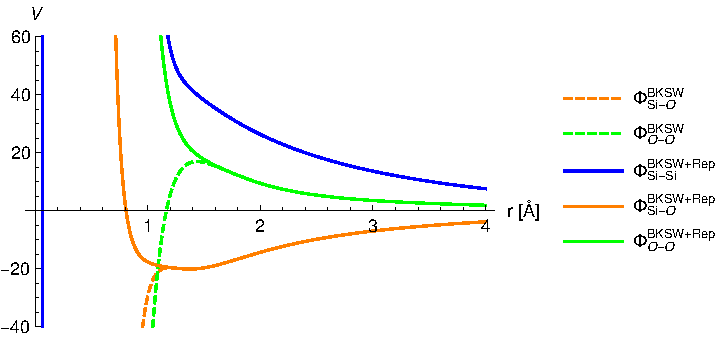
\includegraphics[]{chapters/chapter6/figures/BKSW.pdf}
    \caption{BKS potential with Wolf truncation.}
    \label{fig:BKS-potential}
\end{figure}

\subsection{Sample preparation}


\subsection{Quenching}

%%%%%%%%%%%%%%%%%%%%%%%%%%%%%%%%%%%%%%%%%%%%%
\section{Classical simulations: thermal conductivity}

\subsection{Cepstral analysis}
\paragraph{Dependence on cutoff frequency $f^*$}
(For the chosen sample at experimental density)
(comparison bw normal and vel-renormalized results)

\begin{figure}
    \centering
    \subfigure[\label{fig:csilica-sample-expdens-fstar-100ps}]{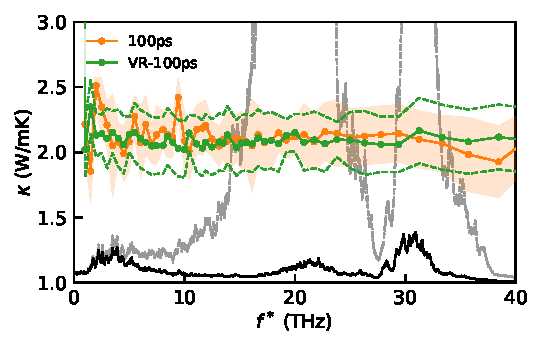
\includegraphics[width=8cm]{chapters/chapter6/figures/silica_expdens_kappa_fstar_VR_100ps.pdf}}
    \subfigure[\label{fig:csilica-sample-expdens-fstar-1ns}]{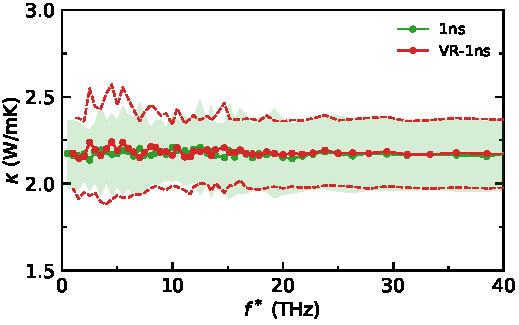
\includegraphics[width=8cm]{chapters/chapter6/figures/silica_expdens_kappa_fstar_VR_1ns.pdf}}
    \subfigure[\label{fig:csilica-sample-expdens-fstar-10ns}]{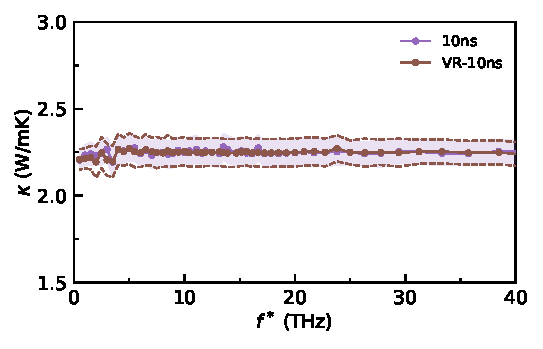
\includegraphics[width=8cm]{chapters/chapter6/figures/silica_expdens_kappa_fstar_VR_10ns.pdf}}
    \caption{Dependence of $\kappa$ on the choice of the cutoff frequency $f^*$, estimated from \emph{one} sample of (a) $100\un{ps}$, (b) $1\un{ns}$, and (c) $10\un{ps}$ of the ``original'' and VR heat flux time series. 
    The original and VR periodograms are reported for reference with grey and black lines, respectively.}
    \label{fig:csilica-sample-expdens-fstar}
\end{figure}
Fig.~\ref{fig:csilica-sample-expdens-fstar} -- stability of $\kappa$ as a function of $f^*$ increases with the length of the trajectory, as its predicted error decreases. The values and errors of $\kappa$ obtained from the VR time series are equivalent to the ones obtained from the original time series, and are slightly more stable with $f^*$. This is probably due to the much smaller power of the power spectrum of the VR heat flux, that may decrease the small artifacts introduced by the low-pass filter applied before resampling. 
Any frequency in the central region of the spectrum can be taken as $f^*$, hence we choose to set $f^*=28\un{THz}$. Conversely, a $f^*$ too small makes $\kappa$ deviate sensibly, due to the fact that the low-pass filter is not strong enough to avoid aliasing effects that modify the spectrum of the resampled time series; instead, a $f^*$ that is too high ($f^*\gtrsim 60\un{THz}$) induces a bias in $\kappa$, due to the fact the log-periodogram diverges to negative values and we start to have problems of numerical precision.

